\documentclass[a4paper,12pt]{extarticle}
\usepackage[utf8x]{inputenc}
\usepackage[T1,T2A]{fontenc}
\usepackage[russian]{babel}
\usepackage{hyperref}
\usepackage{indentfirst}
\usepackage{listings}
\usepackage{color}
\usepackage{here}
\usepackage{array}
\usepackage{multirow}
\usepackage{graphicx}

\usepackage{caption}
\renewcommand{\lstlistingname}{Программа} % заголовок листингов кода

\bibliographystyle{ugost2008ls}

\usepackage{listings}
\lstset{ %
extendedchars=\true,
keepspaces=true,
language=C,						% choose the language of the code
basicstyle=\footnotesize,		% the size of the fonts that are used for the code
numbers=left,					% where to put the line-numbers
numberstyle=\footnotesize,		% the size of the fonts that are used for the line-numbers
stepnumber=1,					% the step between two line-numbers. If it is 1 each line will be numbered
numbersep=5pt,					% how far the line-numbers are from the code
backgroundcolor=\color{white},	% choose the background color. You must add \usepackage{color}
showspaces=false				% show spaces adding particular underscores
showstringspaces=false,			% underline spaces within strings
showtabs=false,					% show tabs within strings adding particular underscores
frame=single,           		% adds a frame around the code
tabsize=2,						% sets default tabsize to 2 spaces
captionpos=t,					% sets the caption-position to top
breaklines=true,				% sets automatic line breaking
breakatwhitespace=false,		% sets if automatic breaks should only happen at whitespace
escapeinside={\%*}{*)},			% if you want to add a comment within your code
postbreak=\raisebox{0ex}[0ex][0ex]{\ensuremath{\color{red}\hookrightarrow\space}},
texcl=true,
inputpath=listings,                     % директория с листингами
}

\usepackage[left=2cm,right=2cm,
top=2cm,bottom=2cm,bindingoffset=0cm]{geometry}

%% Нумерация картинок по секциям
\usepackage{chngcntr}
\counterwithin{figure}{section}
\counterwithin{table}{section}

%%Точки нумерации заголовков
\usepackage{titlesec}
\titlelabel{\thetitle.\quad}
\usepackage[dotinlabels]{titletoc}

%% Оформления подписи рисунка
\addto\captionsrussian{\renewcommand{\figurename}{Рисунок}}
\captionsetup[figure]{labelsep = period}

%% Подпись таблицы
\DeclareCaptionFormat{hfillstart}{\hfill#1#2#3\par}
\captionsetup[table]{format=hfillstart,labelsep=newline,justification=centering,skip=-10pt,textfont=bf}

%% Путь к каталогу с рисунками
\graphicspath{{fig/}}


\begin{document}	% начало документа

% Титульная страница
\begin{titlepage}	% начало титульной страницы

	\begin{center}		% выравнивание по центру

		\large Санкт-Петербургский Политехнический Университет Петра Великого\\
		\large Институт компьютерных наук и технологий \\
		\large Кафедра компьютерных систем и программных технологий\\[6cm]
		% название института, затем отступ 6см
		
		\huge Верификация и анализ программ\\[0.5cm] % название работы, затем отступ 0,5см
		\large Отчет по лабораторной работе №1\\[0.1cm]
		\large Построение поведенческой модели программы по структурной модели\\[5cm]

	\end{center}


	\begin{flushright} % выравнивание по правому краю
		\begin{minipage}{0.25\textwidth} % врезка в половину ширины текста
			\begin{flushleft} % выровнять её содержимое по левому краю

				\large\textbf{Работу выполнил:}\\
				\large Зорин А.Г.\\
				\large {Группа:} 23541/3\\
				
				\large \textbf{Преподаватель:}\\
				\large Ицыксон В.М.

			\end{flushleft}
		\end{minipage}
	\end{flushright}
	
	\vfill % заполнить всё доступное ниже пространство

	\begin{center}
	\large Санкт-Петербург\\
	\large \the\year % вывести дату
	\end{center} % закончить выравнивание по центру

\thispagestyle{empty} % не нумеровать страницу
\end{titlepage} % конец титульной страницы

\vfill % заполнить всё доступное ниже пространство


% Содержание
% Содержание
\renewcommand\contentsname{\centerline{Содержание}}
\tableofcontents
\newpage




\section{Цель работы}
Необходимо построить автоматную модель для следующей задачи:

Горнолоыжный склон, на котором есть две кассы для оплаты, очередь в кассу и очередь на подъемник. Для того, чтобы спуститься со склона необходимо оплатить подъем в одной из двух касс. Человек из очереди подходит к кассе и в течении некоторого времени оплачивает подъем. После оплаты клиенты встают в очередь на подъемник. Далее - подъем на склон. Если клиент поднялся на склон, то считается, что после этого он съедет вниз.

В том случае, когда очередь в кассу занимает больше положенного времени, клиент может уйти. Тогда он не съедет со склона. 

При описании модели стремиться сделать ее масштабируемой по отношению к клиентам и кассам. За стандартную модель были приняты следующие значения: длина очереди - 5, количество касс - 2. 

Проверить следующие утверждения:
\begin{itemize}
\item Все клиенты съедут со склона
\item Все кассы, в конечном итоге, освободятся.
\item Если клиент был в очереди, то, в конечном итоге, он спустится.
\item Ни у кого из клиентов не закончится терпение.
\end{itemize}

\section{Построение модели}
Для реализации заданной модели были построены два конечных автомата, каждый из которых отвечает за поведение отдельного оператора. Такими автоматами являются: клиент и касса. Так же, в системе предусмотрен объект, отвечающий за постановку клиентов в очередь. 

\begin{figure}[H]
	\begin{center}
		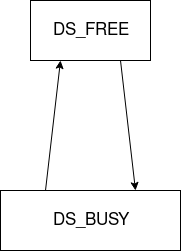
\includegraphics[scale=0.7]{desk}
		\caption{название картинки} 
		\label{pic:desk} % название для ссылок внутри кода
	\end{center}
\end{figure}

\begin{figure}[H]
	\begin{center}
		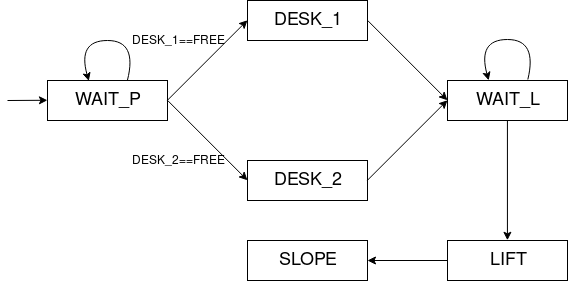
\includegraphics[scale=0.7]{queue}
		\caption{название картинки} 
		\label{pic:queue} % название для ссылок внутри кода
	\end{center}
\end{figure}

\section{Описание модели на языке NuSMV}
C учетом реализации в модель были добавлены несколько проверок на языке LTL и CTL. Описание модели показано в листинге \ref{code:model}

\lstinputlisting[
	label=code:model,
	linerange={1-84},
	caption={Описание задачи},
]{model.smv}
\parindent=1cm


Описание всех спецификаций приведено в листинге \ref{code:spec}.


\lstinputlisting[
	label=code:spec,
	linerange={86-105},
	caption={Описание спецификации},
]{model.smv}
\parindent=1cm

Верификация модели показала, что все спецификации выполняются (листинг \ref{code:tests}).

\lstinputlisting[
	label=code:tests,
	caption={Результаты верификации},
]{tests}
\parindent=1cm

\newpage
\section{Выводы}
В ходе работы была описана и верифицирована модель системы осуществления подъемов и спусков на/со склона. Для описания модели был использован язык NuSMV. А для описания спецификаций --- LTL и CTL формулы.

В результате проделанной работы были выявлены некоторые особенности данного верификатора. К одной из таких особенностей можно отнести соотношение тактов и выполнение шагов автомата (за один такт выполняется один шаг). Так же, плюс данного верификатора --- читаемость кода модели. Однако, существуют и минусы. Например, в данном верификаторе отсутствуют глобальные переменные, что усложняет взаимодействие автоматов на уровне изменения состояний друг друга. Также отсутствуют циклы.

\end{document}
